\maketitle
\tableofcontents
\newpage
\section{(1) Первое задание}
Выберите некоторую функцию (например, $\sin x$, $\cos x$, $\exp x$, $\sh x$, $\ch x$, $\ln x$, \ldots), и некоторую точку $x$ из области определения функции. Найдите значение производной функции в выбранной точке (используя любую формулу численного дифференцирования) с точностью $10^{-3}$, $10^{-6}$. Пользоваться точным значением производной в качестве эталона запрещено.\\[2mm]

Функция, для которой мы будем искать численное значение производной, будет $\sin x$ в точке $x = 0$:


Посчитаем прозводную для $\sin x$, в точке $x_{0} = 1/2$. Для этого воспользуемся разложением в ряд тейлора в окрестности точки $x_{0}$, потом, сравнивая с этим значением, найдем производную с заданной точностью.

\begin{lstlisting}
  f = @(x) sin(x);
  x0 = 1/2;

  syms x
  h = 0.5;

  v = double(subs(taylor(f,x,x0), x0+h) - subs(taylor(f,x,x0), x0-h))


  for eps = [10^-3, 10^-6]
    df = 1;
    while abs(v-df) >= 10^-3
      df = (f(x0+h) - f(x0-h))/(2*h);
      h = h/2;
    end
    df
  end
\end{lstlisting}

\begin{lstlisting}[backgroundcolor=\color{cyan}]
v = 0.841473696062592
df = 0.841470984807897
df = 0.84147347832921
\end{lstlisting}

\section{(2) Второе задание}
Выберите некоторую функцию (например, $\sin x$, $\cos x$, $\exp x$, $\sh x$, $\ch x$, $\ln x$, \ldots) и некоторую точку x из области определения функции. Сравните погрешности у формул с разными порядками погрешностей (например, $y^{'} \approx \frac{y(x+h) - y(x)}{h}$ и $y^{'} \approx \frac{y(x+h) - y(x-h)}{2h}$) для последовательности убывающих шагов (например, $h = \frac{1}{2}, \frac{1}{4}, \frac{1}{8}$). С какими скоростями убывают погрешности для каждой формулы? Дайте теоретическую оценку и подтвердите ответ экспериментом.\\[5mm]
Сравнивать будем две формулы:$y^{'} \approx \frac{y(x+h) - y(x)}{h}$ и $y^{'} \approx \frac{y(x+h) - y(x-h)}{2h}$, с $h = \frac{1}{2}, \frac{1}{4}, \frac{1}{8}$, в точке $x = 1/2$, для функции $\sin x$.\\
$y^{'} \approx \frac{y(x+h) - y(x)}{h} +O(h^{1})$ -- иммеет первый порядок погрешности, а $y^{'} \approx \frac{y(x+h) - y(x-h)}{2h}$ -- второй порядок погрешности

\begin{lstlisting}
f = @(x) sin(x);
x0 = 1/2;
syms x;

R1 = [];
R2 = [];

h = 1/2;
v = double(subs(taylor(f,x,x0), x0+h) - subs(taylor(f,x,x0), x0-h))
n = 10;
h = 1 ./ [2 : n];

for hi = h
  df1 = (f(x0 + hi) - f(x0))/hi;
  df2 = (f(x0 + hi) - f(x0 - hi))/(2*hi);

  R1 = [R1, abs(df1 - v)];
  R2 = [R2, abs(df2 - v)];
end

hold on, grid on;
plot(h, R1, '-*b', h, R2, '-*r')
legend('R1', 'R2')
df1, df2
first_error, second_error
\end{lstlisting}
\begin{figure}[H]
  \caption{}
  \label{fig:plot_1}
  \centering
  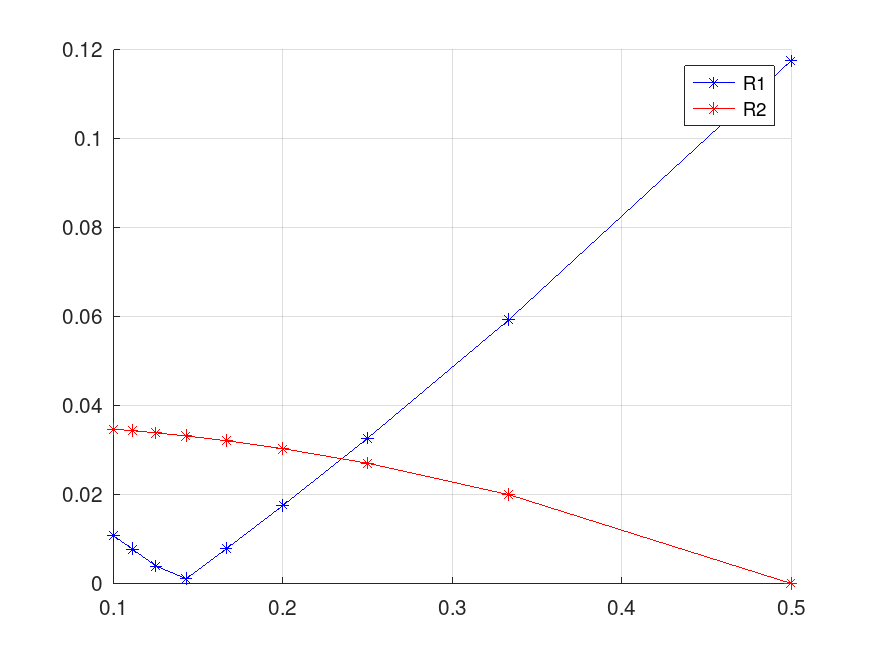
\includegraphics[width=0.9\textwidth]{images/image_2.png}
\end{figure}

\section{(3) Третье задание}
Неустойчивость численного дифференцирования. Выберите некоторую функцию (например, $\sin x$, $\cos x$, $\exp x$, $\sh x$, $\ch x$, $\ln x$, \ldots) и некоторую точку x из области определения функции. Попробуйте применить формулу $y^{'}(x) \approx \frac{y(y+h) - y(x)}{h}$ для стремящейся к нулю последовательности $h = \frac{1}{2}, \frac{1}{4}, \frac{1}{8}, \frac{1}{16}, \ldots$. Будет ли погрешность $\epsilon = \left |y^{'}(x) - \frac{y(x+h) - y(x)}{h} \right |$ монотонно убывать при уменьшении h? Сравните практический и теоритеческий результаты.\\[5mm]
